%%=============================================================================
%% Proof of concept uitwerking
%%=============================================================================

\chapter{\IfLanguageName{dutch}{Proof of Concept uitwerking}{Proof of Concept Implementation}}%
\label{ch:proof of concept implementation}

In dit hoofdstuk wordt de proof of concept ontwikkeld, deze zal aan de requirements voldoen die in Hoofdstuk \ref{ch:requirements analyse} zijn opgesteld. Deze proof of concept zal gebaseerd zijn op de voorbereiding uit Hoofdstuk \ref{ch:proof of concept preparation}.

\section{Netskope Client}

\subsection{Jamf}
Het bedrijf maakt gebruik van de software tool Jamf voor het beheren van de apparaten van de werknemers.

\vspace{2ex}

Jamf is een toonaangevende Mobile Device Management (MDM)-oplossing die specifiek is ontwikkeld voor het beheer van Apple-apparaten binnen organisaties. De oplossing biedt geavanceerde mogelijkheden voor implementatie, beveiliging en beheer, waardoor deze bijzonder geschikt is voor een enterprise-omgeving.  

\vspace{2ex}

Een belangrijk onderdeel van Jamf is de zero-touch implementatie en onboarding, waarbij apparaten direct na het uitpakken automatisch worden geconfigureerd via Apple Business Manager of Apple School Manager.  Dit maakt het mogelijk om de Netskope Client te installeren zonder dat de gebruiker zelf iets hoeft te doen.

\vspace{2ex}

Op het gebied van gedecentraliseerd apparaatbeheer maakt Jamf gebruik van Blueprints, gebaseerd op Apple’s Declarative Device Management, om configuraties, app-installaties en restricties automatisch toe te passen. Smart Groups stellen dynamisch devicegroepen samen op basis van kenmerken zoals OS-versie of locatie, met geautomatiseerde acties om het beheer te stroomlijnen. Via de Self Service+ portal kunnen gebruikers zelf apps en updates installeren, wat gepaard gaat met ingebouwde security-awareness trainingen om het risico op menselijke fouten te verminderen~\autocite{Jamf2025}.

\subsection{Netskope Client}
We kunnen de Netskope Client installeren via Jamf. Op die manier kunnen we de installatie automatiseren zonder manuele tussenkomst van de gebruiker.

\vspace{2ex}

Om de Netskope Client te installeren via Jamf, moeten we de volgende stappen volgen~\autocite{Netskope2025-9}:

\begin{enumerate}
    \item Een nieuwe Jamf policy maken. Dit laat ons toe om de Netskope Client te installeren en om algemene instellingen te configureren.
    \item De Jamf scripts downloaden van de Netskope support website en toevoegen aan de policy.
    \item Netskope Root and Tenant certificaten toevoegen aan de policy. Dit biedt meer beveiliging aan eind gebruikers tijdens de client installatie.
\end{enumerate}

Via Jamf kunnen we dynamische computer groepen maken die bepaalde policies toepast op die specifieke groep. We moeten dan enkel de correcte desbetreffende gebruikers toe voegen aan de groep. Bij die personen zal dan automatisch de Netskope Client geïnstalleerd worden.

\section{Netskope Next Gen Secure Web Gateway (SWG)}
De Netskope SWG is het toegangspunt naar de Netskope cloud, binnen de SWG worden meerdere cruciale componenten ingesteld.

\subsection{Traffic steering}
Bij traffic steering wordt er bepaald welk netwerkverkeer via welke route wordt gestuurd en aan welke beveiligingscontroles het onderworpen wordt. Dit is een essentieel onderdeel van de Netskope-architectuur dat ervoor zorgt dat het juiste verkeer door de juiste beveiligingslaag gaat, afhankelijk van context, gebruiker, apparaat en applicatie.

\subsection{Soorten traffic steering configuratie}

Netskope biedt verschillende methoden voor traffic steering, elk met specifieke toepassingen:

\begin{itemize}
    \item \textbf{All Traffic}: Alle netwerkverkeer van de gebruiker wordt via de Netskope Cloud geleid. Dit biedt de meest uitgebreide beveiliging maar kan impact hebben op de netwerkprestaties.
    \item \textbf{Web Traffic}: Alleen webverkeer (HTTP/HTTPS) wordt via Netskope geleid, terwijl ander verkeer direct naar zijn bestemming gaat.
    \item \textbf{Cloud Apps}: Deze optie stuurt enkel geselcteerde cloud applicaties via Netskope, de rest wordt direct naar de bestemming gestuurd.
    \item \textbf{Private Access Traffic}: Specifiek voor toegang tot private applicaties via ZTNA, waarbij alleen verkeer naar deze applicaties via Netskope wordt geleid.
\end{itemize}
\subsection{Context-gebaseerde configuratie}

De traffic steering-configuratie in Netskope kan worden aangepast op basis van verschillende contextfactoren:

\begin{itemize}
    \item \textbf{Gebruikerslocatie}: Verschillende steering-regels kunnen worden toegepast afhankelijk van of gebruikers zich op kantoor of remote bevinden. Voor dit bedrijf is het zinvol om voor gebruikers op de locaties in Gent, Antwerpen en Leuven een andere configuratie te hanteren dan voor remote medewerkers.
    \item \textbf{Apparaattype en -status}: Beheerde versus niet-beheerde apparaten kunnen verschillende steering-configuraties krijgen, waarbij niet-beheerde apparaten vaak strengere controles ondergaan.
    \item \textbf{Applicatietype}: Verschillende applicaties kunnen verschillende steering-routes volgen. Bijvoorbeeld:
        \begin{itemize}
            \item SaaS-applicaties via Netskope CASB
            \item Private applicaties via Netskope ZTNA
            \item Algemeen webverkeer via Netskope SWG
        \end{itemize}
\end{itemize}
\subsection{Implementatie voor het proof of concept}

Voor onze proof of concept is gekozen voor een gedifferentieerde aanpak:
\begin{itemize}
    \item \textbf{Remote gebruikers}: Voor medewerkers die buiten de kantoorlocaties werken, wordt de ``Web \& Cloud Traffic''-configuratie toegepast, aangevuld met Private Access voor interne applicaties. Hierdoor wordt al het relevante verkeer beveiligd, zonder onnodige latentie voor lokaal verkeer.

    \item \textbf{Kantoorgebruikers}: Voor medewerkers op de kantoorlocaties in Gent, Antwerpen en Leuven wordt een aangepaste configuratie gebruikt waarbij verkeer naar publieke websites en cloudapplicaties via Netskope wordt geleid en verkeer naar interne applicaties direct via de bestaande IPSec-tunnels wordt geleid, en dus niet via Netskope. Dit om optimale prestaties te waarborgen.

    \item \textbf{Testgroep}: Voor de initiële testgroep gebruiken we een voorlopig zowel HTTP als HTTPS verkeer via Netskope, om maximale zichtbaarheid te krijgen voor monitoringdoeleinden, waarbij we nauwlettend de impact op gebruikerservaring volgen. Bij de rest van de gebruikers worden alleen de private applicaties via Netskope geleid.
\end{itemize}
\subsection{Configuratie in Netskope}

De traffic steering-configuratie wordt centraal beheerd in de Netskope-beheerconsole en wordt vervolgens automatisch doorgevoerd naar alle Netskope Clients.

\vspace{2ex}

De specifieke werking van de intelligent traffic steering werkt op basis van DNS, we kunnen binnen de Netskope configuratie een zelfgedefinieerde URL meegeven samen met het te verwachten IP adres. Netskope zal dan deze URL opvragen aan de interne DNS server en het resultaat vergelijken met het ingestelde IP adres. Dit betekent dat we een custom DNS record zullen toevoegen aan de interne DNS server van het bedrijf. Deze DNS server is enkel en alleen bereikbaar op de sites van het bedrijf, en zo zal Netskope kunnen detecteren of een gebruiker op kantoor is of remote.
\begin{listing}[h!]
  \begin{minted}{terraform}
   module "dns_private_net" {
    recordsets = [
        {
        name = "netskope-on-premise.int"
        type = "A"
        ttl  = 300
        records = [
            "1.2.3.4"
        ]
        }
    ]
   }
  \end{minted}
  \caption[Terraform codefragment DNS record]{Terraform codefragment voor het toevoegen van een DNS record.}
\end{listing}

\subsection{Voordelen van intelligente traffic steering}

Een goed geconfigureerde traffic steering-strategie biedt verschillende voordelen:
\begin{itemize}
    \item \textbf{Geoptimaliseerde prestaties}: Alleen noodzakelijk verkeer wordt via de beveiligingscloud geleid
    \item \textbf{Kosteneffectiviteit}: Door niet al het verkeer altijd door de Publisher te sturen, kunnen we minder resources toekennen aan de Publisher. Dit zal ook de kosten verlagen.
    \item \textbf{Flexibiliteit}: De configuratie kan worden aangepast aan veranderende werkomstandigheden
    \item \textbf{Verbeterde gebruikerservaring}: Door lokaal verkeer direct te laten verlopen, wordt latentie geminimaliseerd
\end{itemize}


\section{Netskope Cloud Access Security Broker (CASB)}
Netskope Cloud Access Security Broker (CASB) vormt een essentieel onderdeel van de SASE-architectuur, door zichtbaarheid en controle te bieden over cloudapplicaties. In tegenstelling tot traditionele beveiligingsoplossingen die vaak beperkt zijn tot netwerkperimeters, richt CASB zich specifiek op de beveiliging van cloudapplicaties en de data die daarin wordt verwerkt, ongeacht waar gebruikers zich bevinden.

\subsection{Werking van Netskope CASB}
 
De CASB-functionaliteit van Netskope werkt volgens twee primaire modi:

\begin{itemize}
    \item \textbf{API-modus (Out-of-band)}: In deze modus maakt Netskope gebruik van API-verbindingen met cloudapplicaties om gegevens te scannen die 'at rest' zijn in de cloud. Dit zorgt voor een uitgebreide zichtbaarheid zonder de gebruikersinteractie te beïnvloeden.

    \item \textbf{Forward Proxy-modus (Inline)}: In deze modus wordt alle verkeer naar cloudapplicaties via de Netskope Security Cloud geleid, waardoor real-time inspectie en controle van data in transit mogelijk is.
\end{itemize}

Deze twee modi werken samen om een volledige beveiligingslaag te creëren die zowel statische data als actieve gebruikersinteracties omvat.

\subsection{CASB-implementatie voor bedrijfskritische applicaties}

Voor het proof of concept is er gekozen om CASB-integratie te implementeren voor specifieke bedrijfskritische applicaties:

\begin{itemize}
    \item \textbf{Google Workspace-integratie}:
        \begin{itemize}
            \item \textbf{Google Drive}: Monitoring van documentdeling, identificatie van gevoelige informatie, en controle over wie bestanden mag delen buiten het bedrijf
            \item \textbf{Gmail}: Inspectie van e-mailbijlagen op gevoelige informatie en preventie van data-exfiltratie
            \item \textbf{Google Calendar}: Monitoring van afsprakendeling met externe partijen om datalek via kalenderuitnodigingen te voorkomen
        \end{itemize}
    \item \textbf{Atlassian-productintegratie}:
        \begin{itemize}
            \item \textbf{Confluence}: Bescherming van gevoelige documenten en kennis met controle over externe toegang
            \item \textbf{Jira}: Monitoring van projectgegevens en voorkomen van ongeautoriseerde toegang tot projectinformatie
        \end{itemize}
\end{itemize}

\subsection{Configuratie in het proof of concept}

De configuratie voor de CASB-implementatie omvat de volgende elementen:

\begin{itemize}
    \item \textbf{Applicatie-instances identificeren}: Voor het proof of concept zijn de zakelijke accounts van Google Workspace en Atlassian-producten gedefinieerd en gecategoriseerd.

    \item \textbf{Data en activiteit policies}:
        \begin{itemize}
            \item \textbf{DLP-beleid}: Specifieke regels voor het identificeren van gevoelige gegevens zoals klantendata, interne projectdocumentatie en intellectueel eigendom
            \item \textbf{Activiteitsbeleid}: Configuratie van regels voor specifieke activiteiten zoals downloaden, uploaden, delen en verwijderen
        \end{itemize}

    \item \textbf{Gebruikersprivileges en risicoanalyse}:
        \begin{itemize}
            \item Integratie met Okta voor rolgebaseerde toegangscontrole
            \item Risicoscore toewijzing aan gebruikers op basis van gedrag en activiteitenpatronen
        \end{itemize}
\end{itemize}
\subsection{Specifieke use cases in de implementatie}

De CASB-implementatie is specifiek geconfigureerd voor de volgende use cases:

\begin{itemize}
    \item \textbf{Data-exfiltratie preventie}: Voorkomen dat gevoelige bedrijfsgegevens worden gedeeld met niet-geautoriseerde externe partijen via Google Drive of Confluence.

    \item \textbf{Shadow IT-detectie}: Identificeren van niet-goedgekeurde cloudapplicaties die worden gebruikt voor werkgerelateerde taken.

    \item \textbf{Compliance-monitoring}: Garanderen dat het gebruik van cloudapplicaties voldoet aan interne beleidsregels en externe regelgeving.

    \item \textbf{Anomaliedetectie}: Identificeren van ongebruikelijk gedrag dat kan wijzen op een gecompromitteerd account of insider-bedreiging.
\end{itemize}

\subsection{Voordelen van de CASB-implementatie}

De implementatie van Netskope CASB voor deze cloudapplicaties heeft verschillende significante voordelen opgeleverd:

\begin{itemize}
    \item \textbf{Verbeterde zichtbaarheid}: Volledig inzicht in hoe cloudapplicaties worden gebruikt en hoe data wordt gedeeld
    \item \textbf{Gecontroleerde toegang}: Granulaire controle over wie toegang heeft tot welke bedrijfsinformatie
    \item \textbf{Data-lekkage preventie}: Effectieve bescherming tegen onbedoelde of kwaadwillige data-exfiltratie
    \item \textbf{Compliance-waarborging}: Verzekering dat het gebruik van cloudapplicaties voldoet aan interne en externe regelgeving
    \item \textbf{Verminderd risico}: Proactieve identificatie en mitigatie van beveiligingsrisico's in cloudapplicaties
\end{itemize}

Door de implementatie van Netskope CASB is er een balans gevonden tussen het faciliteren van productieve samenwerking via cloudapplicaties en het waarborgen van de veiligheid van bedrijfskritische gegevens. Deze aanpak sluit naadloos aan bij de bredere SASE-strategie en versterkt het Zero Trust-beveiligingsmodel.

\section{Zero Trust Network Access (ZTNA)}
Netskope Zero Trust Network Access (ZTNA) vormt een essentieel onderdeel van de SASE-architectuur, waarbij de nadruk ligt op het secure-by-design principe. ZTNA biedt toegang tot applicaties zonder het volledige netwerk bloot te stellen, waarbij applicatiespecifieke toegang wordt verleend op basis van identiteit, apparaat en context. 

\vspace{2ex}

Voor ons proof of concept is gekozen voor een integratie met Okta als identiteitsprovider, om een naadloze gebruikerservaring te combineren met robuuste beveiliging.

\subsection{Okta authenticatie en automatische configuratie}

De Okta-integratie binnen Netskope zorgt voor een gestroomlijnde authenticatie en autorisatie:

\begin{itemize}
    \item \textbf{Single Sign-On (SSO)}: Gebruikers kunnen inloggen met hun bestaande Okta-credentials, waardoor een consistente, single sign-on ervaring wordt geboden voor alle applicaties.

    \item \textbf{Groep-gebaseerde configuratie}: De toegewezen rechten en policies worden automatisch bepaald op basis van de Okta-groepen waarvan de gebruiker lid is. Dit elimineert handmatige configuratie per gebruiker en zorgt voor een schaalbare, rolgebaseerde toegangsstructuur.

    \item \textbf{Contextbewuste authenticatie}: Naast gebruikersidentiteit wordt ook rekening gehouden met contextfactoren zoals apparaattype, locatie en compliance-status, om het juiste toegangsniveau te bepalen.

    \item \textbf{Multi-factor authenticatie (MFA)}: Voor gevoelige applicaties wordt aanvullende verificatie vereist, waarbij Okta's MFA-functionaliteit naadloos wordt geïntegreerd in de authenticatieflow.
\end{itemize}

De implementatie in ons proof of concept maakt gebruik van een door Okta gecertificeerde SAML-integratie met Netskope, waarbij gebruikersattributen en groeplidmaatschappen automatisch worden doorgegeven en vertaald naar Netskope-policies.

\subsection{Gebruikerservaring en configuratie}

Vanuit gebruikersperspectief ziet de authenticatie-workflow er als volgt uit:

\begin{enumerate}
    \item De gebruiker logt in op de Netskope Client met dezelfde credentials als voor andere bedrijfsapplicaties
    \item Netskope stuurt de authenticatieaanvraag door naar Okta
    \item Okta verifieert de identiteit en geeft de gebruiker- en groepattributen terug
    \item Op basis van deze attributen worden automatisch de juiste beleidsconfiguraties toegepast
    \item De gebruiker krijgt toegang tot precies die applicaties waarvoor hij/zij geautoriseerd is
\end{enumerate}

Wanneer een gebruiker een actie uitvoert die een real-time policy activeert, kan Netskope dit direct communiceren via een gebruiksvriendelijke pop-up notificatie, zie Figuur \ref{fig:user-alert}. 

\vspace{2ex}

Deze real-time feedback vormt een belangrijk educatief element binnen de SASE-implementatie.
De pop-up notificaties worden getoond wanneer een gebruiker een actie uitvoert die tegen het ingestelde beveiligingsbeleid ingaat, zoals het uploaden van gevoelige documenten naar niet-goedgekeurde clouddiensten of het bezoeken van risicovolle websites. In plaats van simpelweg de actie te blokkeren zonder uitleg, biedt de coaching-functionaliteit context en educatie.
\begin{figure}[h!]
    \centering
    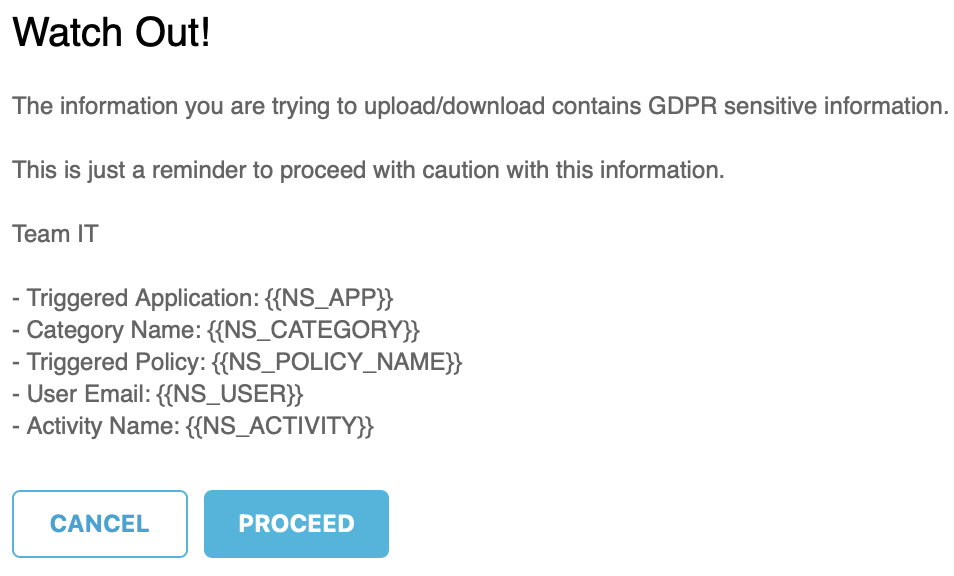
\includegraphics[scale=0.7]{user-warning.png}
    \caption[Netskope ZTNA pop-up notificatie]{Voorbeeld van een pop-up notificatie in Netskope ZTNA}
    \label{fig:user-alert}
\end{figure}

Deze gestroomlijnde workflow zorgt ervoor dat gebruikers slechts de toegang krijgen die ze nodig hebben (least privilege principe), terwijl de administratieve last wordt geminimaliseerd.

\subsection{Real-Time Protection Policies}

Een belangrijke component van de ZTNA-implementatie zijn de Real-Time Protection Policies die continu de toegang en het gebruik van applicaties monitoren en controleren:

\begin{itemize}
    \item \textbf{Applicatiespecifieke controle}: In tegenstelling tot traditionele VPN's wordt toegang verleend tot specifieke applicaties in plaats van het volledige netwerk, waardoor het aanvalsoppervlak aanzienlijk wordt verkleind.

    \item \textbf{Dynamische risicobeoordeling}: De policies evalueren voortdurend het risicoprofiel van de toegangssessie op basis van gebruikersgedrag, apparaatstatus en netwerkcontext. Deze dynamische evaluatie maakt real-time aanpassingen mogelijk indien het risicoprofiel verandert.

    \item \textbf{Granulaire CASB-integratie}: De combinatie van ZTNA met Cloud Access Security Broker (CASB) functionaliteit maakt het mogelijk om diepgaande controle toe te passen op gegevensstromen binnen applicaties, zoals het blokkeren van het uploaden van gevoelige informatie.

    \item \textbf{Continuous monitoring}: Zelfs na de initiële authenticatie blijft het systeem alle interacties monitoren op verdachte activiteiten of afwijkend gedrag, wat kan leiden tot onmiddellijke aanpassing van toegangsrechten of zelfs het verbreken van de sessie.
\end{itemize}

\subsection{Voordelen voor het bedrijf}
De implementatie van Netskope ZTNA met Okta-integratie biedt het bedrijf verschillende belangrijke voordelen:

\begin{itemize}
    \item \textbf{Vereenvoudigde toegang}: Medewerkers ervaren een consistente en gebruiksvriendelijke inlogprocedure voor alle applicaties, ongeacht hun locatie
    \item \textbf{Verhoogde beveiliging}: Het Zero Trust-model verkleint het aanvalsoppervlak en minimaliseert de impact van een potentiële inbreuk
    \item \textbf{Operationele efficiëntie}: Geautomatiseerde groep-gebaseerde configuratie vermindert de administratieve last en het risico op menselijke fouten
    \item \textbf{Verbeterde compliance}: Gedetailleerde logging en controle van toegangsactiviteiten ondersteunt audit- en compliance-vereisten
    \item \textbf{Schaalbaarheid}: Het model schaalt moeiteloos mee met veranderingen in de organisatie, zowel in grootte als structuur
\end{itemize}

Door Netskope ZTNA te implementeren met Okta wordt een belangrijke stap gezet in de transformatie naar een moderne, secure-by-design infrastructuur die medewerkers flexibiliteit biedt zonder onder te hoeven doen aan beveiliging.

\subsection{Bedrijfsapplicaties beveiligen via Okta en Netskope egress IP's}

Een cruciaal onderdeel van de ZTNA-implementatie binnen Netskope is de beveiliging van bedrijfsapplicaties via Okta, waarbij toegang wordt beperkt tot uitsluitend verkeer dat via de Netskope Security Cloud verloopt. Deze aanpak vormt een effectieve extra beveiligingslaag die voorkomt dat gebruikers de Netskope-client kunnen omzeilen, en tevens verzekert dat alle toegang tot bedrijfsapplicaties onderworpen wordt aan de volledige reeks beveiligingscontroles.

\vspace{2ex}

De beveiliging van bedrijfsapplicaties via Okta en Netskope egress IP's werkt volgens het volgende principe:

\begin{enumerate}
    \item \textbf{Netskope egress IP's identificeren}: Elke Netskope Security Cloud POP (Point of Presence) heeft specifieke egress IP-adressen waarvanuit verkeer de Netskope-cloud verlaat richting de doelwebsites en -applicaties. Voor de BE-BRU1 POP, die in onze implementatie wordt gebruikt, zijn deze egress IP's gedocumenteerd en relatief statisch.

    \item \textbf{Okta configureren}: Binnen de Okta-administratie worden de toegangsbeleiden voor bedrijfsapplicaties zodanig geconfigureerd dat ze alleen toegang toestaan vanaf de geautoriseerde Netskope egress IP-adressen. Dit gebeurt via de Network Zones functionaliteit in Okta.

    \item \textbf{Geforceerde routering}: Door deze configuratie wordt alle toegang tot de bedrijfsapplicaties geforceerd via de Netskope Security Cloud, omdat alleen verkeer afkomstig van de Netskope egress IP's wordt toegestaan door Okta.
\end{enumerate}

Als een medewerker op hun Okta dashboard zit en Netskope staat niet aan, dan krijgt men een melding te zien als in Figuur \ref{fig:okta-denied}. Deze zal worden getoond op applicaties waarvoor Netskope ingeschakeld moet zijn.
\begin{figure}[h!]
    \centering
    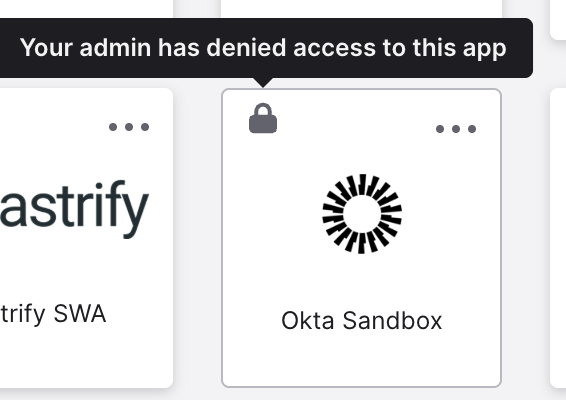
\includegraphics[scale=0.3]{okta-denied.png}
    \caption[Geen Netskope Okta melding]{Voorbeeld van een melding in Okta wanneer Netskope niet is ingeschakeld}
    \label{fig:okta-denied}
\end{figure}

\subsection{Voordelen voor beveiliging}

Deze integratie biedt verschillende belangrijke beveiligingsvoordelen:

\begin{itemize}
    \item \textbf{Volledige inspectie}: Al het verkeer naar bedrijfsapplicaties doorloopt de Netskope beveiligingscontroles, inclusief DLP, malware-scanning en policy enforcement
    \item \textbf{Omzeiling preventie}: Gebruikers kunnen niet bewust of onbewust de beveiligingsmaatregelen omzeilen, wat een belangrijke bescherming biedt tegen shadow IT
    \item \textbf{Contextbewuste toegang}: Netskope kan rijke contextinformatie toevoegen aan de toegangsbesluiten, zoals apparaatgezondheid, gebruikerslocatie en risicobeoordelingen
    \item \textbf{Gecentraliseerde logging}: Alle toegangspogingen worden uniform gelogd binnen het Netskope platform, wat beveiligingsanalyse en incident response verbetert
\end{itemize}

Door bedrijfsapplicaties te beveiligen via Okta en Netskope egress IP's, wordt een belangrijk onderdeel van de ZTNA-architectuur geïmplementeerd dat helpt bij het realiseren van een consistent Zero Trust-model. Waarbij alle toegang wordt geverifieerd, geautoriseerd en gecontroleerd, ongeacht de locatie van de gebruiker of het netwerk waarvan zij verbinding maken.

\section{Netskope Publisher}

De Netskope Publisher vormt een essentiële component binnen de SASE-architectuur door een secure gateway te bieden tussen het Netskope Security Cloud platform en private applicaties in het bedrijfsnetwerk. Anders dan de Netskope Client, die op eindpunten wordt geïnstalleerd, wordt de Publisher geplaatst binnen de netwerkinfrastructuur om private applicaties veilig toegankelijk te maken voor geauthenticeerde gebruikers.

\subsection{Werkingsprincipe van de Netskope Publisher}

De Publisher functioneert volgens een specifiek mechanisme dat de veiligheid van applicatietoegang garandeert:

\begin{enumerate}
    \item De Publisher wordt uitgerold in het netwerksegment waar de applicatieresources zich bevinden. Dit kan een datacenter, cloud-omgeving of een ander netwerkgebied zijn waar private applicaties worden gehost.

    \item Bij opstart registreert de Publisher zich bij de Netskope Security Cloud en authenticeert zichzelf via certificaatauthenticatie, waarbij een beveiligde TLS-tunnel wordt opgebouwd tussen de Publisher en het Netskope-platform.

    \item Wanneer een gebruiker toegang vraagt tot een private applicatie, wordt het verzoek eerst door de Netskope Cloud gevalideerd volgens het bestaande beveiligingsbeleid, inclusief gebruikersidentiteit, apparaatverificatie en contextfactoren.

    \item Bij goedkeuring wordt het verzoek via de beveiligde tunnel doorgestuurd naar de Publisher, die het vervolgens naar de juiste applicatieresource routeert, waarmee een beveiligde end-to-end verbinding tot stand wordt gebracht.
\end{enumerate}

Deze architectuur zorgt ervoor dat private applicaties onzichtbaar blijven voor ongeautoriseerde gebruikers, terwijl ze volledig toegankelijk zijn voor geautoriseerde medewerkers, ongeacht hun locatie of het netwerk van waaruit ze verbinding maken.

\subsection{Implementatie in de proof of concept}

Voor onze proof of concept hebben we de Publisher geïmplementeerd in de GCP region waar de private applicaties worden gehost.

\vspace{2ex}

De implementatie van de Netskope Publisher binnen onze SASE-architectuur heeft geleid tot een aanzienlijke verbetering in zowel de beveiligingsposture als de gebruikerservaring, waarbij medewerkers nu veilig toegang hebben tot bedrijfsapplicaties vanuit elke locatie, zonder de overhead en beperkingen van traditionele VPN-oplossingen.

\section{Netskope Dashboard}
Voor de proof of concept is een Netskope Advanced Analytics dashboard (zie Figuur \ref{fig:dashboard-1}) opgezet om het netwerkverkeer en de beveiliging binnen het bedrijf overzichtelijk op te volgen. Dit dashboard geeft het IT-team in één oogopslag inzicht in wat er gebeurt binnen de Netskope-omgeving, zowel op het vlak van gebruikersacties als beveiligingsincidenten.

\subsection{Dashboard functionaliteiten}
Het dashboard toont onder andere:
\begin{itemize}
    \item \textbf{Device Overview}: Op Figuur \ref{fig:dashboard-1} wordt een overzicht gegeven van alle apparaten die wel of geen verbinding hebben met de Netskope Security Cloud. Hier kan men ook zien bij hoeveel apparaten private access of internet security is ingeschakeld. Ook wordt er weergegeven hoeveel gebruikers manueel hun Netskope hebben uitgeschakeld.
    \item \textbf{Malware}: Op Figuur \ref{fig:dashboard-1} wordt weergegeven welke malware er is gedetecteerd en de specifieke details van deze malware. Ook worden malsites weergegeven, dit zijn websites die gebruikt worden om malware te verspreiden. Uiteindelijk wordt er een trendlijn weergegeven van de aantal malware en malsites detecties over de gekozen periode.
    \item \textbf{User Behavior Analytics (UBA)}: Op Figuur \ref{fig:dashboard-2} wordt een grote flow matrix weergegeven van alle gedetecteerde gebruikersactiviteiten. Deze flows worden geleid naar het platform waar deze activiteiten zijn gedetecteerd.
    \item \textbf{AI Usage}: Op Figuur \ref{fig:dashboard-3} wordt een overzicht weergegeven van de AI-gebruik binnen het bedrijf. Er wordt getoond hoeveel gebruikers AI gebruiken en welke AI services worden gebruikt. Verder wordt er getoond wat de grootste services zijn en welke gevolgen deze hebben gegeven, dit kan gaan van een user coaching die wordt gegeven of een allow. Binnen de user coaching wordt er dan ook getoond welke actie de gebruiker heeft genomen.
\end{itemize}

\begin{figure}[h!]
    \centering
    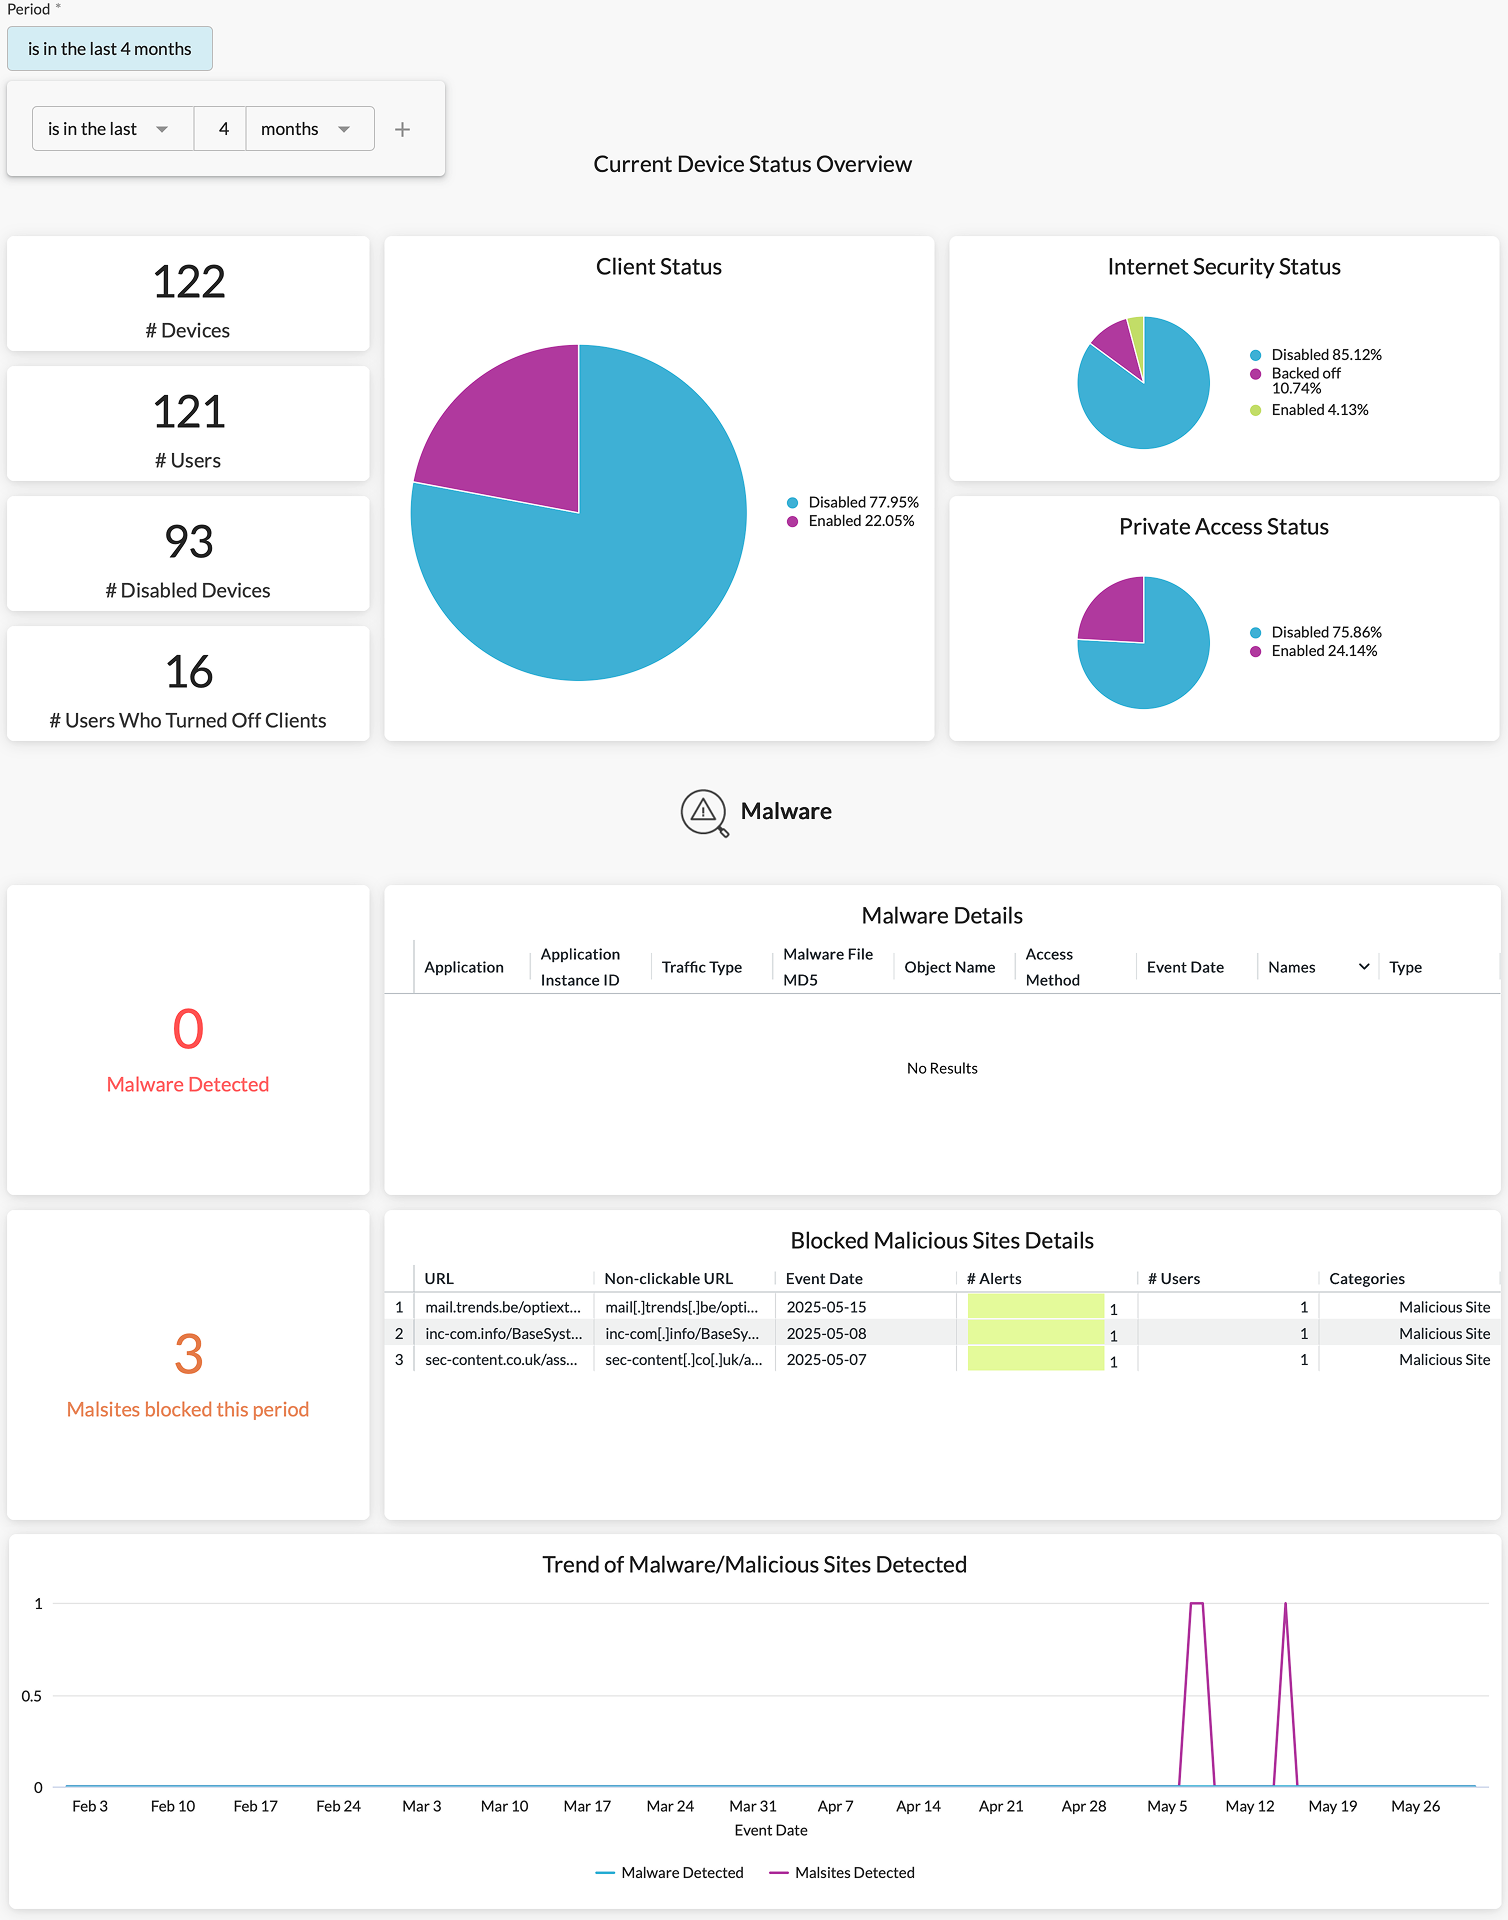
\includegraphics[width=\textwidth]{dashboard-1.png}
    \caption[Netskope Advanced Analytics dashboard - Deel 1]{Eerste deel van het Netskope Advanced Analytics dashboard}
    \label{fig:dashboard-1}
\end{figure}
\begin{figure}[h!]
    \centering
    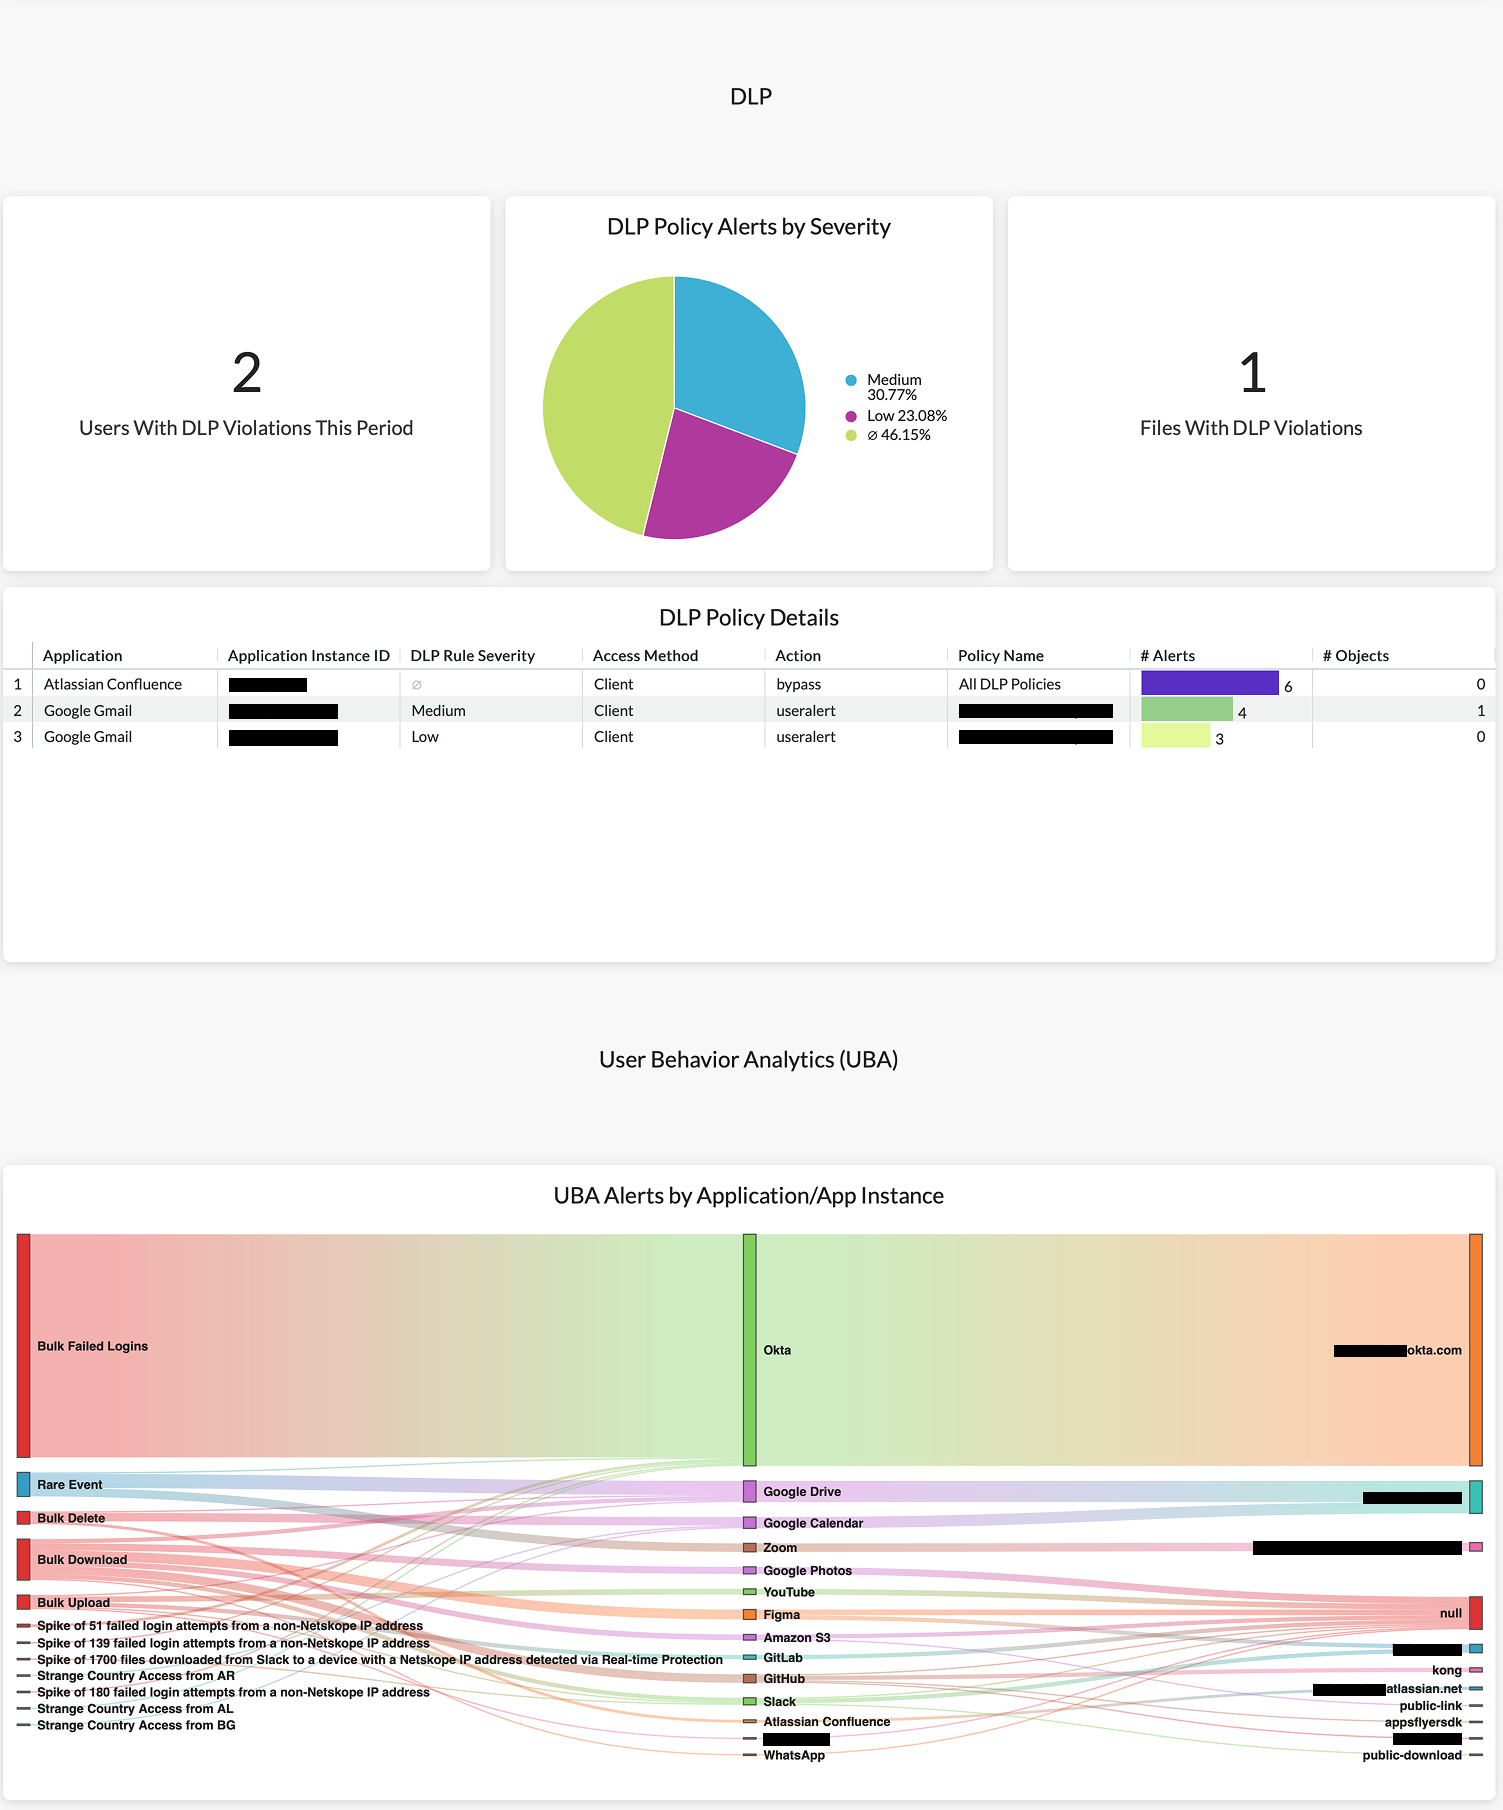
\includegraphics[width=\textwidth]{dashboard-2.png}
    \caption[Netskope Advanced Analytics dashboard - Deel 2]{Tweede deel van het Netskope Advanced Analytics dashboard}
    \label{fig:dashboard-2}
\end{figure}
\begin{figure}[h!]
    \centering
    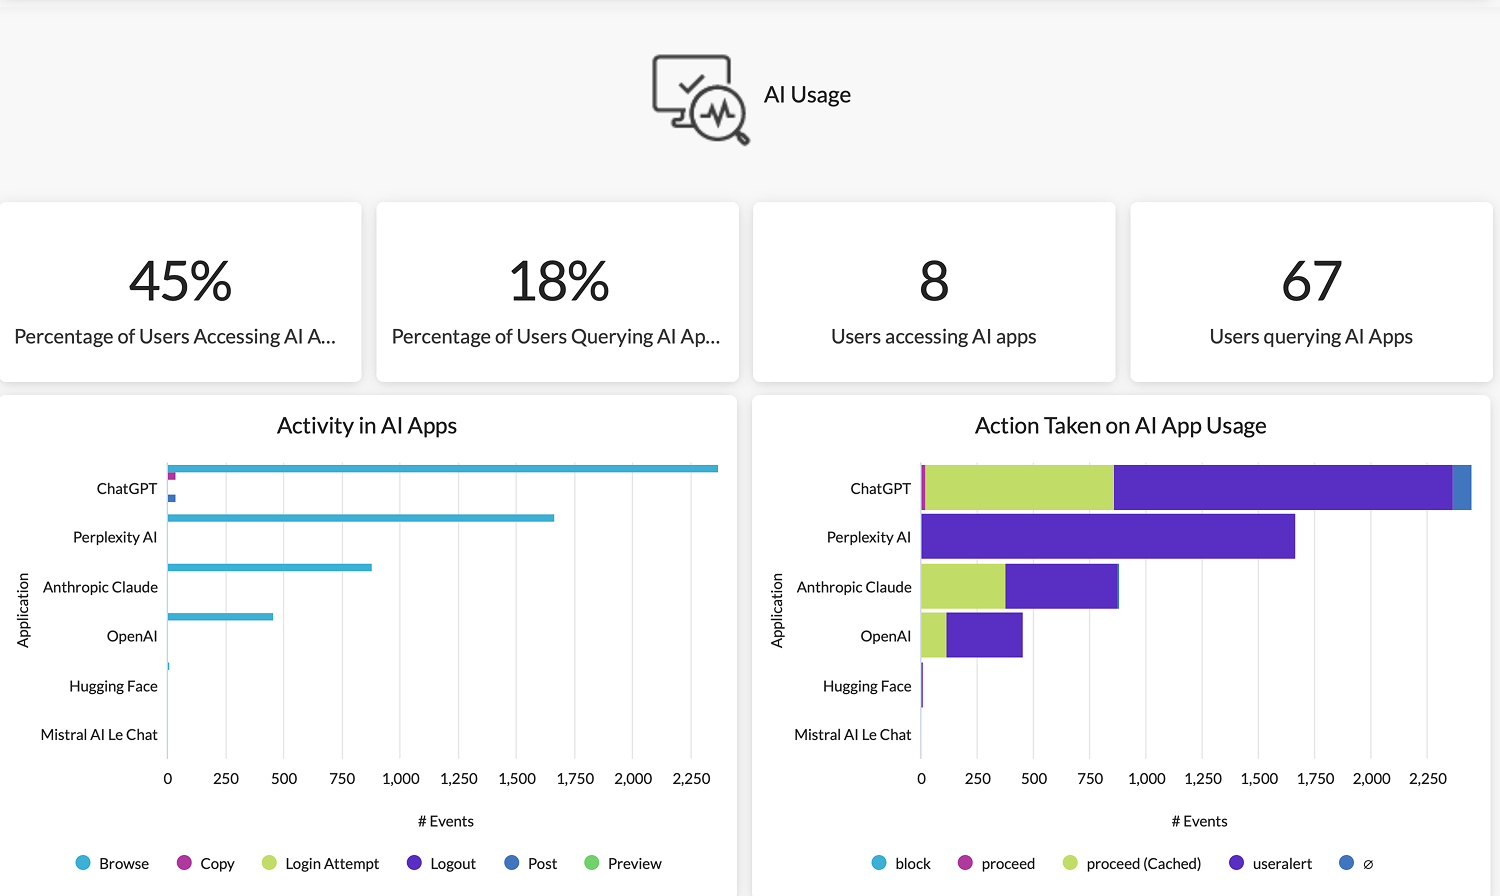
\includegraphics[width=\textwidth]{dashboard-3.png}
    \caption[Netskope Advanced Analytics dashboard - Deel 3]{Derde deel van het Netskope Advanced Analytics dashboard}
    \label{fig:dashboard-3}
\end{figure}

Het dashboard wordt dagelijks gebruikt om trends te volgen, incidenten te onderzoeken en het beleid waar nodig aan te passen. Zo kan het team bijvoorbeeld bij een toename van geblokkeerde uploads naar Google Drive nagaan of de policy moet worden aangepast of dat er extra uitleg aan gebruikers nodig is.

\vspace{2ex}

Door deze inzichten kan het bedrijf sneller reageren op problemen en blijft de controle over de beveiliging en het gebruik van cloudapplicaties behouden. Het dashboard zorgt voor meer overzicht, snellere detectie van problemen en maakt het makkelijker om de Netskope-omgeving goed te beheren. Het helpt het IT-team om beter onderbouwde beslissingen te nemen en de beveiliging continu te verbeteren.

\vspace{2ex}

Het dashboard wordt wekelijks overgebracht aan het IT-team via mail. Dit zorgt ervoor dat het team altijd op de hoogte is van de laatste ontwikkelingen en trends binnen de Netskope-omgeving, en stelt hen in staat om proactief te reageren op eventuele problemen of veranderingen.